
\documentclass[lineno]{jfm}

\usepackage{graphicx}
%\usepackage{epstopdf,epsfig}
\usepackage{newtxtext}
\usepackage{newtxmath}
\usepackage{natbib}
\usepackage{hyperref}
\hypersetup{
    colorlinks = true,
    urlcolor   = blue,
    citecolor  = black,
}
\newtheorem{lemma}{Lemma}
\newtheorem{corollary}{Corollary}
\newcommand{\RomanNumeralCaps}[1]
\linenumbers


% {\MakeUppercase{\romannumeral #1}}

\title{Guidelines for authors}

\author{Alan N. Jones\aff{1}
  \corresp{\email{JFMEditorial@cambridge.org}},
  H.-C. Smith\aff{1}
 \and J.Q. Long\aff{2}}

\affiliation{\aff{1}STM Journals, Cambridge University Press, The Printing House, Shaftesbury Road, Cambridge CB2 8BS, UK
\aff{2}DAMTP, Centre for Mathematical Sciences, Wilberforce Road, Cambridge CB3 0WA, UK}

\begin{document}
\maketitle

\begin{abstract}
This file contains instructions for authors planning to submit a paper to the {\it Journal of Fluid Mechanics}. These instructions were generated in {\LaTeX} using the JFM class file, and the source files for these instructions can be used as a template for submissions. The present paragraph appears in the \verb}abstract} environment. All papers should feature a single-paragraph abstract of no more than 250 words, which provides a summary of the main aims and results.  In addition to the figures in the main article a graphical abstract is now required. It will be used as a small thumbnail in the table of contents and on the abstract page, so multiple panels are not suitable and will be rejected. Please confirm that you have included an image to accompany your abstract, which will be used as the graphical abstract for manuscripts published in 2020. The image must be of aspect ratio 1.2:1 (e.g. 6cm x 5cm) and should be submitted in GIF or high resolution JPEG format (300 dpi). Unless very large, vector graphics are preferred to ensure image sharpness regardless of sizing. If you do not have the copyright to the image, please ensure you have permission to reuse the figure. Captions are not required. Text is actively discouraged, but if it must be used, it should be legible in a small thumbnail (2.4cmx2cm) presented in the table of contents. All graphical abstract images will be considered for a JFM cover selection by the JFM Panel. Please note that we publish 24 covers in a year.
\end{abstract}

\begin{keywords}
Authors should not enter keywords on the manuscript, as these must be chosen by the author during the online submission process and will then be added during the typesetting process (see \href{https://www.cambridge.org/core/journals/journal-of-fluid-mechanics/information/list-of-keywords}{Keyword PDF} for the full list).  Other classifications will be added at the same time.
\end{keywords}

{\bf MSC Codes }  {\it(Optional)} Please enter your MSC Codes here

\section{How to submit to the \emph{Journal of Fluid Mechanics}}
\label{sec:intro}

 Authors must submit using the online submission and peer review system \href{https://mc.manuscriptcentral.com/jfm} {Scholar One} (formerly Manuscript Central). If visiting the site for the first time, users must create a new account by clicking on `register here'. Once logged in, authors should click on the `Corresponding Author Centre', from which point a new manuscript can be submitted, with step-by-step instructions provided. Authors must at this stage specify whether the submission is a {\it JFM Paper}, or a {\it JFM Rapids} paper (see \S4 for more details). In addition, authors must specify an editor to whom the paper will be submitted from the drop-down list provided. Note that all editors exclusively deal with either {\it JFM Paper} or {\it JFM Rapids} (clearly indicated on the list), so please ensure that you choose an editor accordingly. Corresponding authors must provide a valid ORCID ID in order to submit a manuscript, either by linking an existing ORCID profile to your ScholarOne account or by creating a new ORCID profile. Once your submission is completed you will receive an email confirmation. Book reviews should not be submitted via the online submission site, but should instead be submitted by email to anne.juel@manchester.ac.uk.
% * <ajohns@cambridge.org> 2018-06-14T10:05:40.418Z:
%
% ^.

\section{Rules of submission}\label{sec:rules_submission}
 Submission of a paper implies a declaration by the author that the work has not previously been published, that it is not being considered for publication elsewhere and that it has not already been considered by a different editor of the Journal.  If you have uploaded your manuscript via the arXiv function, then please include your E-print Number during the submission process.

\section {Authors responsibilites}
 Authors need to declare in their covering letter to the Editor and during the online submission process whether their manuscript had previously been considered for publication in the {\it Journal of Fluid Mechanics}.  Questions and declarations to that effect must be answered truthfully.
Editors, referees, readers and publishers have the right to assume that submitted (and published) manuscripts do not contain scientific dishonesty or fraud comprising, for example, fictitious or manipulated data, plagiarised material (either from previous work of the authors or that of other persons), reference omissions, false priority statements, `hidden' multiple publication of the same data or incorrect authorship.  Authors must not breach any copyright.  The {\it Journal of Fluid Mechanics} uses the iThenticate software to detect instances of plagiarism in manuscripts submitted to it.
\subsection {Transparency and Openness Promotion (TOP)}
 The overarching policy of the {\it Journal of Fluid Mechanics} is that research articles should contain sufficient information to allow others to understand, replicate and verify findings, and compare them with alternative studies. We therefore require that whenever possible:

 {\bf Understanding} - Articles should be written and will be assessed for clarity, both of the execution of the research and for its outcomes and conclusions.

 {\bf Replication} - All information required to replicate the study must be provided, within the body of the paper and/or publicly accessible repositories.  Examples of what is required include but are not limited by:
\begin{itemize}
\item for analytical studies, the mathematically complete set of equations and boundary conditions, any theorems relied upon, appropriately referenced;
\item for numerical studies, the mathematically complete set of equations and boundary conditions, sufficient descriptions of the algorithms or packages used to solve them, appropriately referenced, and the resolution used with respect to the independent variables;
\item for laboratory experiments, the dimensions and construction of any apparatus, the materials used including their relevant physical properties, the protocol adopted for the running of the experiments, the measurement tools used including their resolution and accuracy, including appropriate calibration standards;
\item for field studies, the raw data collected or used, any protocols or tools used to access the data (e.g. data-mining tools) or to process it.
\end{itemize}
{\bf Verification} -  Most studies can be verified or falsified provided that sufficient detail is given for them to be replicated (see above).  Where data is manipulated (for example, bringing together multiple data sets by scaling) the raw (dimensional) data relating to the primary measurements (laboratory) or outputs (numerical) should be provided together with the protocols or tools used to process them.

{\bf Comparison} - All graphical information should be supplemented with numerical data or precise algorithms to reproduce it.  For example, data points should be provided in a spreadsheet and curves should be defined either explicitly with an equation or as resulting from a precisely defined algorithm.


\section{Types of paper}\label{sec:types_paper}
\subsection{Standard papers}
 Regular submissions to JFM are termed `standard papers'. Note that such papers must contain original research. Papers should be written in a concise manner; though JFM has no page limit, each paper will be judged on its own merits, and those deemed excessive in length will be rejected or will require significant revision.
\subsection{JFM Rapids}
 {\it JFM Rapids} is devoted to the rapid publication of short, high-impact papers across the full range of fluid mechanics. Manuscripts submitted as {\it JFM Rapids}  must be strictly 10 or fewer printed pages, and must be submitted in {\LaTeX} using the jfm.cls class file, so as to ensure that they meet the page limit and to expedite their production.  As with standard papers, the principal and over-riding objective is to publish papers of the highest scientific quality.

Once a paper is submitted, reviewers are asked to provide reports with a short turnaround.  In order to be accepted for publication in {\it JFM Rapids}, such papers must be strongly endorsed by the referees and should require only minor revisions to improve clarity, usually without recourse to a second round of reviewing. In this case, and at the discretion of the editor, some additional pages may be allowed to address specific points raised by the reviewers, such as the addition of an extra figure or some explanatory text.

Papers that are rejected having been submitted to Rapids are rejected on behalf of the whole Journal and may not be submitted for consideration by another associate editor of JFM, whether for Rapids or as a Standard paper.

In cases where the editor, guided by the reviewers, judges that a paper has merit but requires substantial revision that will require significant reviewing, a decision of `revise and resubmit' will be given. On re-submission, such papers will be handled as standard JFM papers and if accepted will not subsequently appear as {\it JFM Rapids}.

{\it JFM Rapids} will be published online within one month of final acceptance.  They will appear within a designated section on the {\it Journal of Fluid Mechanic}s website.  Each {\it Rapid} will be cited and indexed as a JFM article but with a distinctive {\it Rapids} identifier, and will be assigned to a JFM volume.

\subsection{JFM Perspectives}
 Review papers are published under {\it JFM Perspectives } and are by invitation only.
%\pagebreak

\section{File types}\label{sec:filetypes}
 Authors are strongly encouraged to compose their papers in {\LaTeX}, using the \href{https://www.cambridge.org/core/journals/journal-of-fluid-mechanics/information/instructions-contributors} {jfm.cls} style file and supporting files provided, with the \href{https://www.cambridge.org/core/journals/journal-of-fluid-mechanics/information/instructions-contributors} {jfm-instructions.tex} file serving as a template (please note that this is mandatory for {\it JFM Rapids}). A PDF of the {\LaTeX} file should then be generated and submitted via the submission site. For the review process the pdf file should be no more than 10MB. There is no need to submit the {\LaTeX} source files alongside the PDF, but upon provisional acceptance of the paper, the {\LaTeX} source files, along with individual figure files and a PDF of the final version, will need to be submitted for typesetting purposes.
Authors may also compose standard papers in Word, though this will lead to the paper spending a longer period in production. If using Word, please note that equations must NOT be converted to picture format and the file must be saved with the option `make equation editable'. All submitted video abstract files should be formatted as MP4 (H.264). MP4 has full compatibility across commonly used browsers, whereas other video formats will only work on selected browsers. This will ensure the greatest possible dissemination of this work.
\section{Preparing your manuscript}
 Authors should write their papers clearly and concisely in English, adhering to JFM's established style for mathematical notation, as provided in Section \ref{notstyle}. We encourage the submission of online supplementary material alongside the manuscript where appropriate (see Section \ref{online}). Metric units should be used throughout and all abbreviations must be defined at first use, even those deemed to be well known to the readership. British spelling must be used, and should follow the \textit{Shorter Oxford English Dictionary}.

\begin{figure}
  \centerline{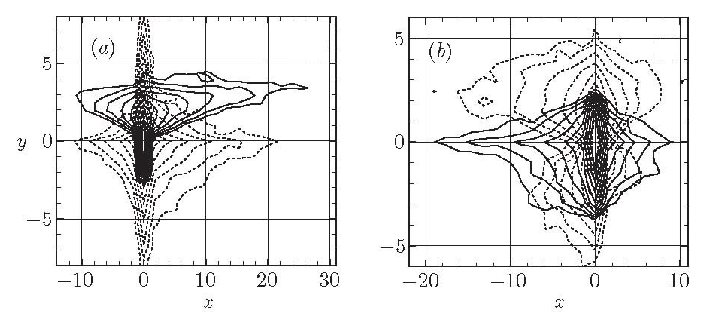
\includegraphics{Fig1}}% Images in 100% size
  \caption{Trapped-mode wavenumbers, $kd$, plotted against $a/d$ for
    three ellipses:\protect\\
    ---$\!$---,
    $b/a=1$; $\cdots$\,$\cdots$, $b/a=1.5$.}
\label{fig:ka}
\end{figure}


\subsection{Figures}
 All authors need to acquire the correct permissions and licences to reproduce figures, which should be submitted with the production files. Further information on applying for permission to reuse figures can be found \href{https://www.cambridge.org/core/journals/journal-of-fluid-mechanics/information/request-permissions}{here}.  Images should be submitted in EPS or high-resolution TIFF format (1200 dpi for lines, 300 dpi for halftone and colour in RGB format, and 600 dpi for a mixture of lines and halftone) and all labels should be editable. Unless very large, vector graphics are preferred to ensure image sharpness regardless of sizing. The minimum acceptable width of any line is 0.5pt. Each figure should be accompanied by a single caption, to appear beneath, and must be cited in the text. Figures should appear in the order in which they are first mentioned in the text and figure files must be named accordingly (`Abstract.eps, Fig1.eps', `Fig2a.tiff', etc) to assist the production process (and numbering of figures should continue through any appendices). Words \textit {figure 1, table 1 and movie  1} should be lower case. For example see figures \ref{fig:ka} and \ref{fig:kd}.
 Failure to follow figure guidelines may result in a request for resupply and a subsequent delay in the production process. Note that {\em all} figures will be relabelled by the typesetter, so please ensure all figure labels are carefully checked against your originals when you receive your proofs.

\begin{figure}
  \centerline{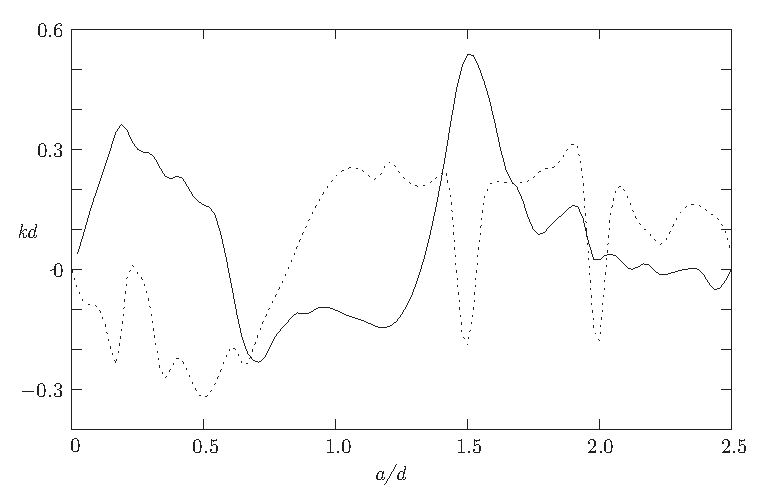
\includegraphics{Fig2}}
  \caption{The features of the four possible modes corresponding to
  (\textit{a}) periodic\protect\\ and (\textit{b}) half-periodic solutions.}
\label{fig:kd}
\end{figure}

\subsection{Tables}
 Tables, however small, must be numbered sequentially in the order in which they are mentioned in the text. Words \textit {table 1, table 2} should be lower case throughout.
 See table \ref{tab:kd} for an example.

\begin{table}
  \begin{center}
\def~{\hphantom{0}}
  \begin{tabular}{lccc}
      $a/d$  & $M=4$   &   $M=8$ & Callan \etal \\[3pt]
       0.1   & 1.56905 & ~~1.56~ & 1.56904\\
       0.3   & 1.50484 & ~~1.504 & 1.50484\\
       0.55  & 1.39128 & ~~1.391 & 1.39131\\
       0.7   & 1.32281 & ~10.322 & 1.32288\\
       0.913 & 1.34479 & 100.351 & 1.35185\\
  \end{tabular}
  \caption{Values of $kd$ at which trapped modes occur when $\rho(\theta)=a$.}
  \label{tab:kd}
  \end{center}
\end{table}


\subsection{Online supplementary material}\label{online}
 Relevant material which is not suitable for inclusion in the main article, such as movies or numerical simulations/animations, can be uploaded as part of the initial submission. Movies must be submitted in .mp4 format and have the file designation of `Movie'.  Each movie must be numbered in the order they are mentioned and titled movie 1, movie 2 etc and accompanied by a separate caption. To ensure maths terms display correctly they should be bounded by \textcolor{red}{ \$\$} and written in TeX, e.g. movie 1. Side view of numerical Schlieren contours from case E1N at {\$$z=Lz/2$\$}. Each movie should be no more than 50MB. Upon publication these materials will then be hosted online alongside the final published article. Likewise, should there be detailed mathematical relations, tables or figures which are likely to be useful only to a few specialists or take up excessive space in the article, these should also be published online as supplementary material [designated as `Other supplementary material']. Note that supplementary material is published `as is', with no further intervention made during the Production process, all `draft' information should be removed.

\section{Editorial decisions}
\subsection{Revision}
 If a revision is requested, you should upload revised files following the same procedure as for submitting a new paper. You begin by clicking on `Manuscripts with decision' in your Corresponding Author Centre, and then on `Create a revision'. (Note that if you abandon the process before completing the submission, to continue the submission, you must click on `Revised manuscripts in draft'.) There is a new first page showing the decision letter and a space for your reply to the reviewer's/editor's comments. You also have the opportunity at this stage to upload your reply to the comments as  separate files. All the values filled in on original submission are displayed again. The ID number of the paper will be appended `.R1'. Also note that if a manuscript is submitted as a {\it JFM Rapid}, but requires substantial revision, it will be re-designated as a standard paper, and the ID and paper type will be amended to reflect this.

\subsection{Provisional acceptance}
 If the paper is accepted as suitable for publication you will be sent a provisional acceptance decision. This enables you to upload the final files required for production:
(1) the final PDF or word version of the paper, designated as a `Main Document';
(2) any source files (see section \ref{sec:filetypes}) which must be designated as `Production Files' and uploaded as a single .zip or .tar file;
(3) a completed author publishing agreement form which is available to download at \href{https://www.cambridge.org/core/journals/journal-of-fluid-mechanics/information/author-publishing-agreement}{Cambridge Core}. For Open Access there is a one-off fee, further information can be found at \href{https://www.cambridge.org/core/journals/journal-of-fluid-mechanics/information/jfm-open-access-faqs} {JFM open access - FAQs}. If your research is publicly funded and your organisation comes under one of Cambridge University Press's Read and Publish agreements you may be entitled to free Open Access. Please check your eligibility \href{https://www.cambridge.org/core/services/open-access-policies/read-and-publish-agreements}{here}.



\subsection{Acceptance}
 On receipt of the production files you will be sent an email indicating completion of the acceptance process.

\section{Publication process}
 Once a paper has been accepted for publication and the source files have been uploaded, the manuscript will be sent to Cambridge University Press for copyediting and typesetting, and will be assigned a digital object identifier (doi). When the proof is ready, authors will receive an email alert containing a link to the PDF of the proof, and instructions for its correction and return. It is imperative that authors check their proofs closely, particularly the equations and figures, which should be checked against the accepted file, as the production schedule does not allow for corrections at a later stage. Once ready, papers will be published online on \href{https://www.cambridge.org/core/journals/journal-of-fluid-mechanics}{Cambridge Core} in the current `open' volume.  Each volume will be kept open for approximately two weeks. Note that the PDF published online is the Version of Record and no further alterations/corrections to this document will be allowed. The corresponding author is emailed a link to the published article when it is published online.

\section{Corrigenda}
 The Journal will publish corrigenda that alter significant conclusions made in a paper.  Such corrigenda should be submitted to an associate editor, who will consider the submission similarly to a new paper and may consult referees if appropriate.  When published, corrigenda are clearly linked with the original articles to which they refer, and the articles to them.

\indent The Journal does not normally publish corrigenda to amend typographical errors, so it is extremely important that authors make very careful checks of their manuscript at every stage, including the reading of proofs, prior to publication.



\section{Obtaining help}
 Technical support for the online submission system is available by clicking on the `Get Help Now' link at the top-right corner of each page of the submission site. Any other questions relating to the submission or publication process should be directed to the JFM Editorial Assistant, Mrs Amanda Johns, at JFMEditorial@cambridge.org.

\section{Cambridge Author Services - in partnership with American Journal Experts}
 We suggest that authors whose first language is not English have their manuscripts checked by a native English speaker before submission. This is optional but will help to ensure that any submissions that reach peer review can be judged exclusively on academic merit. Further information can be found at \href{https://www.cambridge.org/core/services/authors/language-services} {Language services}, and we suggest that authors make contact as appropriate. Please note that use of language editing services is voluntary and at the author\textquotesingle s own expense. Use of these services does not guarantee that the manuscript will be accepted for publication nor does it restrict the author to submitting to a Cambridge-published journal.

\section{Notation and style}\label{notstyle}
 Generally any queries concerning notation and journal style can be answered by viewing recent pages in the Journal. However, the following guide provides the key points to note. It is expected that Journal style and mathematical notation will be followed, and authors should take care to define all variables or entities upon first use. Also note that footnotes are not normally accepted.  Abbreviations must be defined at first use, glossaries or lists/tables of abbreviations are not permitted.

\subsection{Mathematical notation}
\subsubsection{Setting variables, functions, vectors, matrices etc}
\begin{itemize} \label{sec:MathNot}
\item {\bf Italic font} should be used for denoting variables, with multiple-letter symbols avoided except in the case of dimensionless numbers such as $\Rey$, $\Pran$ and $\Pen$ (Reynolds, Prandtl, and P\'eclet numbers respectively, which are defined as \verb}\Rey}, \verb}\Pran} and \verb}\Pen} in the template).\\
\item {\bf Upright Roman font} (or upright Greek where appropriate) should be used for:\\
\begin {enumerate}
\item (vI) label, e.g.  T. t (transpose)\\
\item Fixed operators: sin, log, d, $\Delta$, exp etc.\\
\item Constants: i ($\sqrt{-1}$), $\upi$ (defined as \verb}\upi}),e  etc.\\
\item Special Functions: $\Ai$, $\Bi$ (Airy functions, defined as \verb}\Ai} and \verb}\Bi}), $\Real$ (real part, defined as \verb}\Real}), $\Imag$ (imaginary part, defined as \verb}\Imag}), etc.\\[-4pt]
\item Physical units: cm, s, etc.\\[-4pt]
\item Abbreviations: c.c. (complex conjugate), h.o.t. (higher-order terms), DNS, etc.\\[-4pt]
\end {enumerate}
\item {\bf Bold italic font} (or bold sloping Greek) should be used for vectors (with the centred dot for a scalar product also in bold): $\boldsymbol{i \cdot j}$\\[-4pt]
\item {\bf Bold sloping sans serif font}, defined by the \verb}\mathsfbi} macro, should be used for tensors and matrices: $\mathsfbi{D}$ \\[-4pt]
\item {\bf Calligraphic font} (for example $\mathcal{G}$, $\mathcal{R}$) can be used as an alternative to italic when the same letter denotes a different quantity use \verb}\mathcal} in \LaTeX)
\end{itemize}

\subsubsection{Other symbols}  Large numbers  that are not scientific powers should not include commas, but should use a non-breaking space, and use the form 1600 or 16 000 or 160 000.
Use \textit{O} to denote `of the order of', not the \LaTeX\ $\mathcal{O}$.

The product symbol ($\times$) should only be used to denote multiplication where an equation is broken over more than one line, to denote a cross product, or between numbers . The $\boldsymbol {\cdot}$ symbol should not be used, except to denote a scalar product of vectors specifically.

\section{Citations and references}
All papers included in the References section must be cited in the article, and vice versa. Citations should be included as, for example ``It has been shown
\citep{Rogallo81} that...'' (using the {\verb}\citep} command, part of the natbib package) ``recent work by \citet{Dennis85}...'' (using {\verb}\citet}).
The natbib package can be used to generate citation variations, as shown below.\\
\verb#\citet[pp. 2-4]{Hwang70}#:\\
\citet[pp. 2-4]{Hwang70} \\
\verb#\citep[p. 6]{Worster92}#:\\
\citep[p. 6]{Worster92}\\
\verb#\citep[see][]{Koch83, Lee71, Linton92}#:\\
\citep[see][]{Koch83, Lee71, Linton92}\\
\verb#\citep[see][p. 18]{Martin80}#:\\
\citep[see][p. 18]{Martin80}\\
\verb#\citep{Brownell04,Brownell07,Ursell50,Wijngaarden68,Miller91}#:\\
\citep{Brownell04,Brownell07,Ursell50,Wijngaarden68,Miller91}\\
\citep{Briukhanovetal1967}\\
\cite{Bouguet01}\\
\citep{JosephSaut1990}\\
The References section can either be built from individual \verb#\bibitem# commands, or can be built using BibTex. The BibTex files used to generate the references in this document can be found in the zip file \href{http://journals.cambridge.org/data/relatedlink/jfm-ifc.zip}{jfm-ifcs}.\\
Where there are up to ten authors, all authors' names should be given in the reference list. Where there are more than ten authors, only the first name should appear, followed by {\it {et al.}}

JFM discourages citations of manuscript posted on social media sites (such as ResearchGate) or on pre-print servers (e.g. ArXiv), that have not been peer-reviewed or published in journals.

\backsection[Supplementary data]{\label{SupMat}Supplementary material and movies are available at \\https://doi.org/10.1017/jfm.2019...}

\backsection[Acknowledgements]{Acknowledgements may be included at the end of the paper, before the References section or any appendices. Several anonymous individuals are thanked for contributions to these instructions.}

\backsection[Funding]{Please provide details of the sources of financial support for all authors, including grant numbers. For example, "This work was supported by the National Science Foundation (grant number XXXXXXX)". Multiple grant numbers should be separated by a comma and space, and where research was funded by more than one agency the different agencies should be separated by a semi-colon, with 'and' before the final funder. Grants held by different authors should be identified as belonging to individual authors by the authors' initials. For example, "This work was supported by the Deutsche Forschungsgemeinschaft (A.B., grant numbers XXXX, YYYY), (C.D., grant number ZZZZ); the Natural Environment Research Council (E.F., grant number FFFF); and the Australian Research Council (A.B., grant number GGGG), (E.F., grant number HHHH)". \\
Where no specific funding has been provided for research, please provide the following statement: "This research received no specific grant from any funding agency, commercial or not-for-profit sectors." }

\backsection[Declaration of interests]{A {\bf Declaration of interests} statement is now mandatory in the manuscript PDF. Please included a statement in your manuscript at the end of the main text with regards to any known competing financial interests or personal relationships that could appear to have influenced the work reported in this paper. These must also be declared in your covering letter to the Editor. Please note that if there are no conflicts of interest, the declaration in your PDF should read as follows: {\bf Declaration of Interests}. The authors report no conflict of interest.}

\backsection[Data availability statement]{The data that support the findings of this study are openly available in [repository name] at http://doi.org/[doi], reference number [reference number].}

\backsection[Author ORCID]{Authors may include the ORCID identifers as follows.  F. Smith, https://orcid.org/0000-0001-2345-6789; B. Jones, https://orcid.org/0000-0009-8765-4321}

\backsection[Author contributions]{Authors may include details of the contributions made by each author to the manuscript, for example, ``A.G. and T.F. derived the theory and T.F. and T.D. performed the simulations.  All authors contributed equally to analysing data and reaching conclusions, and in writing the paper.''}

\section{Appeals process}

The {\it Journal of Fluid Mechanics} has an appeal procedure which provides authors with the opportunity to respond to the editorial decision on their manuscript, should they think that their manuscript was treated in an unfair manner during the peer-review process.  Authors have the right to appeal to the Editor or Editor-in-Chief against any decision taken on their manuscript at any stage.  An appeal will be considered at the direction of the Editorial Board of the Journal.
\subsection {How do I appeal?}
\begin{itemize}
\item[{\bf Step 1.}] Requests to have the decision on a submission re-considered should be made in the first instance to the Associate Editor who handled the submission and made the decision.  Send a rebuttal letter to the Associate Editor, explaining clearly why you disagree with the decision on your manuscript and including a detailed response to any points of contention in the referees' reports.  The Associate Editor will consider your appeal and either invite you to submit a revised paper or confirm the original decision.
\item[{\bf Step 2.}]In case you remain unsatisfied with the Associate Editor's response after Step 1 or at any stage should you consider that your submission was treated unfairly, you should send a letter of appeal to the Editor-in-Chief via the Journal email (JFMEditorial@cambridge.org). Your letter should explain clearly the grounds for your appeal.
\item[{\bf Step 3.}] The Editor-in-Chief will consider the grounds of your appeal and if he considers there to be a {\it prima facie} case to consider may assign one of the Deputy Editors to consider the appeal in detail.  All appeal requests are handled on a case by case basis and the Deputy Editor's or Editor-in-Chief's decision is final.  Appeals are normally considered on the basis of whether or not the process of review was conducted appropriately.  Papers will not routinely be sent for further review.
\end{itemize}

\appendix

\section{}\label{appA}
 This appendix contains sample equations in the JFM style. Please refer to the {\LaTeX} source file for examples of how to display such equations in your manuscript.

\begin{equation}
  (\nabla^2+k^2)G_s=(\nabla^2+k^2)G_a=0
  \label{Helm}
\end{equation}

\begin{equation}
  \bnabla\bcdot\boldsymbol{v} = 0,\quad \nabla^{2}P=
    \bnabla\bcdot(\boldsymbol{v}\times \boldsymbol{w}).
\end{equation}

\begin{equation}
  G_s,G_a\sim 1 / (2\upi)\ln r
  \quad \mbox{as\ }\quad r\equiv|P-Q|\rightarrow 0,
  \label{singular}
\end{equation}

\begin{equation}
\left. \begin{array}{ll}
\displaystyle\frac{\p G_s}{\p y}=0
  \quad \mbox{on\ }\quad y=0,\\[8pt]
\displaystyle  G_a=0
  \quad \mbox{on\ }\quad y=0,
 \end{array}\right\}
  \label{symbc}
\end{equation}


\begin{equation}
  -\frac{1}{2\upi} \int_0^{\infty} \gamma^{-1}[\mathrm exp(-k\gamma|y-\eta|)
   + \mathrm exp(-k\gamma(2d-y-\eta))] \cos k(x-\xi)t\:\mathrm{d} t,
   \qquad 0<y,\quad \eta<d,
\end{equation}

\begin{equation}
  \gamma(t) = \left\{
    \begin{array}{ll}
      -\mathrm{i}(1-t^2)^{1/2}, & t\le 1 \\[2pt]
      (t^2-1)^{1/2},         & t>1.
    \end{array} \right.
\end{equation}

\[
  -\frac{1}{2\upi}
   \pvi B(t)\frac{\cosh k\gamma(d-y)}{\gamma\sinh k\gamma d}
   \cos k(x-\xi)t\:\mathrm{d} t
\]

\begin{equation}
  G = -\frac{1}{4}\mathrm{i} (H_0(kr)+H_0(kr_1))
    - \frac{1}{\upi} \pvi\frac{\mathrm{e}^{-\kgd}}%
    {\gamma\sinh\kgd} \cosh k\gamma(d-y) \cosh k\gamma(d-\eta)
\end{equation}

Note that when equations are included in definitions, it may be suitable to render them in line, rather than in the equation environment: $\boldsymbol{n}_q=(-y^{\prime}(\theta),
x^{\prime}(\theta))/w(\theta)$.
Now $G_a=\squart Y_0(kr)+\Gat$ where
$r=\{[x(\theta)-x(\psi)]^2 + [y(\theta)-y(\psi)]^2\}^{1/2}$ and $\Gat$ is
regular as $kr\ttz$. However, any fractions displayed like this, other than $\thalf$ or $\squart$, must be written on the line, and not stacked (ie 1/3).

\begin{eqnarray}
  \ndq\left(\frac{1}{4} Y_0(kr)\right) & \sim &
    \frac{1}{4\upi w^3(\theta)}
    [x^{\prime\prime}(\theta)y^{\prime}(\theta)-
    y^{\prime\prime}(\theta)x^{\prime}(\theta)] \nonumber\\
  & = & \frac{1}{4\upi w^3(\theta)}
    [\rho^{\prime}(\theta)\rho^{\prime\prime}(\theta)
    - \rho^2(\theta)-2\rho^{\prime 2}(\theta)]
    \quad \mbox{as\ }\quad kr\ttz . \label{inteqpt}
\end{eqnarray}

\begin{equation}
  \frac{1}{2}\phi_i = \frac{\upi}{M} \sumjm\phi_j K_{ij}^a w_j,
  \qquad i=1,\,\ldots,\,M,
\end{equation}
where
\begin{equation}
  K_{ij}^a = \left\{
    \begin{array}{ll}
      \p G_a(\theta_i,\theta_j)/\p n_q, & i\neq j \\[2pt]
      \p\Gat(\theta_i,\theta_i)/\p n_q
      + [\rho_i^{\prime}\rho_i^{\prime\prime}-\rho_i^2-2\rho_i^{\prime 2}]
      / 4\upi w_i^3, & i=j.
  \end{array} \right.
\end{equation}


\refstepcounter{equation}
$$
  \rho_l = \lim_{\zeta \rightarrow Z^-_l(x)} \rho(x,\zeta), \quad
  \rho_{u} = \lim_{\zeta \rightarrow Z^{+}_u(x)} \rho(x,\zeta)
  \eqno{(\theequation{\mathit{a},\mathit{b}})}\label{eq35}
$$

\begin{equation}
  (\rho(x,\zeta),\phi_{\zeta\zeta}(x,\zeta))=(\rho_0,N_0)
  \quad \mbox{for}\quad Z_l(x) < \zeta < Z_u(x).
\end{equation}


\begin{subeqnarray}
  \tau_{ij} & = &
    (\overline{\overline{u}_i \overline{u}_j}
    - \overline{u}_i\overline{u}_j)
    + (\overline{\overline{u}_iu^{SGS}_j
    + u^{SGS}_i\overline{u}_j})
    + \overline{u^{SGS}_iu^{SGS}_j},\\[3pt]
  \tau^\theta_j & = &
    (\overline{\overline{u}_j\overline{\theta}}
    - \overline{u}_j \overline{\theta})
    + (\overline{\overline{u}_j\theta^{SGS}
    + u^{SGS}_j \overline{\theta}})
    + \overline{u^{SGS}_j\theta^{SGS}}.
\end{subeqnarray}

\begin{equation}
\setlength{\arraycolsep}{0pt}
\renewcommand{\arraystretch}{1.3}
\slsQ_C = \left[
\begin{array}{ccccc}
  -\omega^{-2}V'_w  &  -(\alpha^t\omega)^{-1}  &  0  &  0  &  0  \\
  \displaystyle
  \frac{\beta}{\alpha\omega^2}V'_w  &  0  &  0  &  0  &  \mathrm{i}\omega^{-1} \\
  \mathrm{i}\omega^{-1}  &  0  &  0  &  0  &  0  \\
  \displaystyle
  \mathrm{i} R^{-1}_{\delta}(\alpha^t+\omega^{-1}V''_w)  &  0
    & -(\mathrm{i}\alpha^tR_\delta)^{-1}  &  0  &  0  \\
  \displaystyle
  \frac{\mathrm{i}\beta}{\alpha\omega}R^{-1}_\delta V''_w  &  0  &  0
    &  0  & 0 \\
  (\mathrm{i}\alpha^t)^{-1}V'_w  &  (3R^{-1}_{\delta}+c^t(\mathrm{i}\alpha^t)^{-1})
    &  0  &  -(\alpha^t)^{-2}R^{-1}_{\delta}  &  0  \\
\end{array}  \right] .
\label{defQc}
\end{equation}

\begin{equation}
\etb^t = \skew2\hat{\etb}^t \exp [\mathrm{i} (\alpha^tx^t_1-\omega t)],
\end{equation}
where $\skew2\hat{\etb}^t=\boldsymbol{b}\exp (\mathrm{i}\gamma x^t_3)$.
\begin{equation}
\mbox{Det}[\rho\omega^2\delta_{ps}-C^t_{pqrs}k^t_qk^t_r]=0,
\end{equation}

\begin{equation}
 \langle k^t_1,k^t_2,k^t_3\rangle = \langle
\alpha^t,0,\gamma\rangle
\end{equation}

\begin{equation}
\boldsymbol{f}(\theta,\psi) = (g(\psi)\cos \theta,g(\psi) \sin \theta,f(\psi)).
\label{eq41}
\end{equation}

\begin{eqnarray}
f(\psi_1) = \frac{3b}{\upi[2(a+b \cos \psi_1)]^{{3}/{2}}}
  \int^{2\upi}_0 \frac{(\sin \psi_1 - \sin \psi)(a+b \cos \psi)^{1/2}}%
  {[1 - \cos (\psi_1 - \psi)](2+\alpha)^{1/2}}\mathrm{d}x,
\label{eq42}
\end{eqnarray}
\begin{eqnarray}
g(\psi_1) & = & \frac{3}{\upi[2(a+b \cos \psi_1)]^{{3}/{2}}}
  \int^{2\upi}_0 \left(\frac{a+b \cos \psi}{2+\alpha}\right)^{1/2}
  \left\{ \astrut f(\psi)[(\cos \psi_1 - b \beta_1)S + \beta_1P]
  \right. \nonumber\\
&& \mbox{}\times \frac{\sin \psi_1 - \sin \psi}{1-\cos(\psi_1 - \psi)}
  + g(\psi) \left[\left(2+\alpha - \frac{(\sin \psi_1 - \sin \psi)^2}
  {1- \cos (\psi - \psi_1)} - b^2 \gamma \right) S \right.\nonumber\\
&& \left.\left.\mbox{} + \left( b^2 \cos \psi_1\gamma -
  \frac{a}{b}\alpha \right) F(\frac{1}{2}\upi, \delta) - (2+\alpha)
  \cos\psi_1 E(\frac{1}{2}\upi, \delta)\right] \astrut\right\} \mathrm{d} \psi,
\label{eq43}
\end{eqnarray}
\begin{equation}
\alpha = \alpha(\psi,\psi_1) = \frac{b^2[1-\cos(\psi-\psi_1)]}%
  {(a+b\cos\psi) (a+b\cos\psi_1)},
  \quad
  \beta - \beta(\psi,\psi_1) = \frac{1-\cos(\psi-\psi_1)}{a+b\cos\psi}.
\end{equation}


\begin{equation}
\left. \begin{array}{l}
\displaystyle
H(0) = \frac{\epsilon \overline{C}_v}{\tilde{v}^{{1}/{2}}_T
(1- \beta)},\quad H'(0) = -1+\epsilon^{{2}/{3}} \overline{C}_u
+ \epsilon \skew5\hat{C}_u'; \\[16pt]
\displaystyle
H''(0) = \frac{\epsilon u^2_{\ast}}{\tilde{v}^{{1}/{2}}
_T u^2_P},\quad H' (\infty) = 0.
\end{array} \right\}
\end{equation}

\begin{lemma}
Let $f(z)$ be a trial \citet[][pp.~231--232]{Batchelor59} function defined on $[0,1]$.  Let $\varLambda_1$ denote
the ground-state eigenvalue for $-\mathrm{d}^2g/\mathrm{d} z^2=\varLambda g$,
where $g$ must satisfy $\pm\mathrm{d} g/\mathrm{d} z+\alpha g=0$ at $z=0,1$
for some non-negative constant~$\alpha$.  Then for any $f$ that is not
identically zero we have
\begin{equation}
\frac{\displaystyle
  \alpha(f^2(0)+f^2(1)) + \int_0^1 \left(
  \frac{\mathrm{d} f}{\mathrm{d} z} \right)^2 \mathrm{d} z}%
  {\displaystyle \int_0^1 f^2\mathrm{d} z}
\ge \varLambda_1 \ge
\left( \frac{-\alpha+(\alpha^2+8\upi^2\alpha)^{1/2}}{4\upi} \right)^2.
\end{equation}
\end{lemma}

\begin{corollary}
Any non-zero trial function $f$ which satisfies the boundary condition
$f(0)=f(1)=0$ always satisfies
\begin{equation}
  \int_0^1 \left( \frac{\mathrm{d} f}{\mathrm{d} z} \right)^2 \mathrm{d} z.
\end{equation}
\end{corollary}


\bibliographystyle{jfm}
\bibliography{jfm}
%Use of the above commands will create a bibliography using the .bib file. Shown below is a bibliography built from individual items.

%\bibliographystyle{jfm}
%\bibliography{jfm2esam}

%\begin{thebibliography}{99}
%
%\expandafter\ifx\csname natexlab\endcsname\relax
%\def\natexlab#1{#1}\fi
%\expandafter\ifx\csname selectlanguage\endcsname\relax
%\def\selectlanguage#1{\relax}\fi
%
%\bibitem[Batchelor (1971)]{Batchelor59}
%{\sc Batchelor, G.K.} 1971 {Small-scale variation of convected quantities like temperature in turbulent fluid part1, general discussion and the case of small conductivity}, {\it J. Fluid Mech.}, {\bf 5}, pp. 3-113-133.
%
%\bibitem [Bouguet (2008)]{Bouguet01}
%{\sc Bouguet, J.-Y} 2008 Camera Calibration Toolbox for Matlab {\url{http://www.vision.caltech.edu/bouguetj/calib_doc/}}.
%
% \bibitem[Briukhanovetal et al (1967)] {Briukhanovetal1967}
%{\sc Briukhanov, A. V.,   Grigorian, S. S., Miagkov,  S. M., Plam, M. Y.,   I. E. Shurova, I. E.,   Eglit, M. E. and Yakimov, Y. L.} 1967
%{On some new approaches to the dynamics of snow avalanches},
%{\it Physics of Snow and Ice,  Proceedings of the International Conference on Low Temperature Science}
%{Vol 1} pp. 1221--1241 {Institute of Low Temperature Science, Hokkaido University, Sapporo, Hokkaido, Japan}.
%
%\bibitem[Brownell (2004)]{Brownell04}
% {\sc Brownell,  C.J.  and Su,  L.K.} 2004  {Planar measurements of differential diffusion in turbulent jets}, {\it AIAA Paper},  pp. 2004-2335.
%
%\bibitem[Brownell and Su (2007)] {Brownell07}
%  {\sc Brownell, C.J. and  Su, L.K.} 2007 {Scale relations and spatial spectra in a differentially diffusing jet}, {\it AIAA Paper}, pp 2007-1314.
%
%\bibitem [Dennis (1985)] {Dennis85}
% {\sc  Dennis, S.C.R.} 1985 {Compact explicit finite difference approximations to the Navier--Stokes equation},  { In \it Ninth Intl Conf. on Numerical Methods in Fluid Dynamics},  {ed Soubbaramayer and J.P. Boujot},  {Vol 218}, {\it Lecture Notes in Physics}, pp. 23-51. Springer.
%
%\bibitem [Edwards et al. (2017)]{EdwardsVirouletKokelaarGray2017}
%{\sc Edwards, A. N., Viroulet, S., Kokelaar, B. P. and Gray, J. M. N. T.} 2017 Formation of levees, troughs and elevated channels by avalanches on erodible slopes {\it J. Fluid Mech.}, {\bf 823}, pp. 278-315.
%
%\bibitem[Hwang et al (1970)] {Hwang70}
% {\sc Hwang,  L.-S.  and  Tuck, E.O.} 1970 On the oscillations of harbours of arbitrary shape {\it J.~Fluid Mech.}, {\bf42}, pp 447-464.
%
%\bibitem[Josep and Saut (1990)] {JosephSaut1990}
% {\sc Joseph, Daniel D. and Saut, Jean Claude} 1990 Short-wave instabilities and ill-posed initial-value problems {\it Theoretical and Computational Fluid Dynamics}, {\bf 1},  pp.191--227,  {\url{http://dx.doi.org/10.1007/BF00418002}}.
%
%\bibitem[Worster (1992)] {Worster92}
%{ \sc  Worster, M.G.} 1992 The dynamics of mushy layers {\it Interactive dynamics of convection and solidification},
%{(ed. S.H. Davis and H.E. Huppert and W. Muller and M.G. Worster)}, pp. 113--138 {Kluwer}.
%
%\bibitem[Koch(1983)] {Koch83}
%{\sc Koch, W.} 1983 Resonant acoustic frequencies of flat plate cascades {\it J.~Sound Vib.}, {\bf 88}, pp. 233-242.
%
%\bibitem[Lee(1971)] {Lee71}
%{\sc Lee,  J.-J.}  1971 Wave-induced oscillations in harbours of arbitrary geometry {\it J.~Fluid Mech.}, {\bf 45}, pp. 375-394.
%
%\bibitem[Linton and  Evans (1992)] {Linton92}
% {\sc  Linton, C.M. and  Evans, D.V.} 1992 The radiation and scattering of surface waves by a vertical circular cylinder in a channel {\it Phil.\ Trans.\ R. Soc.\ Lond.}, {\bf 338}, pp. 325-357.
%
%\bibitem [Martin(1980] {Martin80}
% {\sc  Martin, P.A.} 1980 On the null-field equations for the exterior problems of acoustics {\it Q.~J. Mech.\ Appl.\ Maths},{\bf 33}, pp. 385--396.
%
%\bibitem [Rogallo(1981)] {Rogallo81}
% {\sc Rogallo,  R.S.} 1981 Numerical experiments in homogeneous turbulence  { {\it Tech. Rep.} 81835}  {NASA Tech.\ Mem}.
%
%\bibitem[Ursell(1950)] {Ursell50}
%{\sc  Ursell, F.} 1950 Surface waves on deep water in the presence of a submerged cylinder i {\it Proc.\ Camb.\ Phil.\ Soc.}, {\bf 46}, pp.141--152.
%
%\bibitem[Wijngaarden (1968)]{Wijngaarden68}
%{\sc van Wijngaarden, L.} 1968 On the oscillations Near and at resonance in open pipes {\it J.~Engng Maths},{\bf 2}, pp. 225--240.
%
%\bibitem[Miller (1991)]{Miller91}
%{ \sc  Miller, P.L.} 1991 Mixing in high Schmidt number turbulent jets {school {PhD thesis}} {California Institute of Technology}.
%
%\end{thebibliography}

%% End of file `jfm2esam.bib'.

\end{document}
